%!TEX encoding = UTF-8 Unicode
\chapter{Schedule of Future Work}
\label{sec:Schedule}

Future work is scheduled as follows:
\begin{itemize}[noitemsep]
  \item February, 1st - February, 21th: Choice of applications and specifications of test target scenarios;
  \item February, 22th - March, 21th: Communication between fog nodes at the same level;
  \item March, 22th - May, 30th: Static Optimization;
  \item May, 23th - June, 5th: Preliminary results;
  \item June, 6th - July, 31th: Mobility implementation;
  \item August, 1st - September, 25th: Optimization with mobility;
  \item September, 18th - October, 8th: Final results;
  \item March, 1st - October, 10th: Write the dissertation about the work performed.
\end{itemize}
\noindent\tab The Gantt diagram corresponding to the thesis schedule is shown in Figure \ref{fig:schedule}.
\begin{figure}[h]
	\centering
	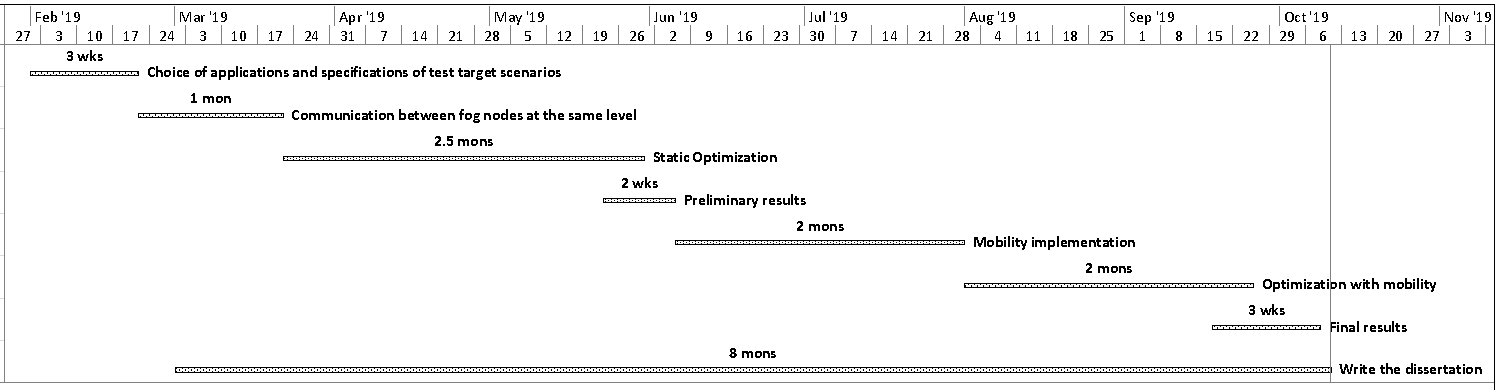
\includegraphics[width=\textwidth]{images/schedule/schedule.pdf}
	\caption{Gantt diagram for the thesis schedule.}
	\label{fig:schedule}
\end{figure}